\documentclass[12pt]{article}
%\documentclass[12pt]{proc}
\usepackage{graphicx}    % includes epsf
\usepackage{hyperref}
\usepackage{booktabs}
\usepackage{multirow}
\usepackage{siunitx}
\usepackage{threeparttable}
\usepackage{tabularx}
\newcommand{\ra}[1]{\renewcommand{\arraystretch}{#1}}

\begin{document}
%\onecolumn
\title{Beam parameters for the Hall-B RG-C run during June 2022 through March 2023}
\author{}
\date{\today}
\maketitle

Hall-B Run Group C is scheduled to run from June 8, 2022, to March 14, 2023. in experimental Hall B. The CLAS12 is a multipurpose detector system based on a toroidal (forward detector) and a solenoid (central  detector) superconducting magnets. The detector system includes Cherenkov Counters, Drift Chambers, Scintillator Counters, Silicon-strip detectors, Micro-mega gas detectors, and Calorimeters. In this run period CLAS12 will be used in its standard detector and shielding configuration with the Forward tagger ON. In August the run will be briefly interrupted  to remove Forward tagger and install the Large M\o{}ller cone. For the RG-C, the CLAS12 polarized solid target will be used, adding a 1 K evaporation refrigerator and microwave system to CLAS12. 

The CLAS12 polarized target will be located in the center of the 5~T solenoid magnet, and will consist of a 2~cm diameter Kel-F cell, with 0.05~mm foil aluminum windows, containing beads of solid NH$_3$ or ND$_3$ target material. This cell is held in a bath of liquid helium at near 1~K at the end of a 3~m long horizontal refrigerator, which allows the beam to pass through its center. Upon entering the refrigerator through an Al window, the beam will travel 3~m through a tube containing low pressure (1~torr) helium gas, before passing through the aluminum window of the target bath. The beam then passes through 2~cm of super-fluid helium before entering and after exiting the 5~cm long target cell. Finally, the beam will exit the refrigerator through an aluminum bath window, aluminum inner vacuum window and aluminum outer vacuum window. The areal density of NH$_3$(+He) cell is 3(+0.3)~g/cm$^2$. The areal density of ND$_3$(+He) cell is 3.5(+0.3)~g/cm$^2$. This corresponds to roughly 8\% of radiation length

In this run period we will use longitudinally polarized electron beam of $\ge$10.5~GeV (5-pass). The luminosity during the run will be ~10$^{35}$~cm$^{-2}$s$^{-1}$, the nominal design luminosity for CLAS12. Typical production beam currents will be below 10~nA. The beam will be rastered over the target area with a spiral pattern. For the empty target runs the beam current could be up to 100~nA for several hours. There will also be used for calibration purposes ancillary C, CH$_2$ and CD$_2$ targets with the thickness of the order of 3~g/cm$^2$. The beam current on these targets will be less than 10~nA. The first week of the run 1-pass beam will be used for experiment commissioning .

To be able to achieve a higher polarization of ND$_3$ material it will be irradiated by 50~nA beam current for 3--6 hours. This procedure will be repeated four times over the run period. During irradiation CLAS12 detectors will be turned off. During running with beam above 15 nA at 11 GeV (160~W), the Hall B beam stopper (a 30~cm long, water cooled-copper absorber) will be positioned before the Faraday Cup to prevent overheating. 
For the initial beam tuning or after extended down time ($>$8 hours) and for M\o{}ller runs, the beam will be directed into the beam dump in the Hall B Tagger dipole yoke.



The details of all components, such as windows and cells, are shown on the beam line drawing, including thicknesses and locations.  The beam line layout is shown in Figures \ref{fig:beamline1} - \ref{fig:beamline4}.


To minimize a heat load and radiation damages to the target material and maintain uniform and high polarization the beam will be rastered. The raster pattern will be a constant linear velocity  spiral with the radius up to 9~mm. The beam rastering will be done by two pairs of dipole magnets. The first pair is located between 2C24A BPM and the tagger magnet. The second pair is located between the 2H01 BPM and the target. To prevent rapid target depolarization in case of the stopped rastering the FSD from the the raster magnets' currents will be implemented.

The requirements for beam parameters for RG-C run are summarized in Table~\ref{tab:beam_par}

 \begin{table}[htb]
\caption{Required beam parameters.}\label{tab:beam_par}
\centering
 \begin{tabular}{|c|c|l|}
\hline
Parameter & Requirement &Comments \\ \hline 
Energy (GeV) & 10.5+, 2   & 5, 1 pass  \\  \hline
$\delta$p/p & $\sim 2\times 10^{-4}$ & \\ \hline 
Current (nA) & $\le 10$ &up to 100 nA on empty target  \\  \hline
$\sigma_{xy}$ ($\mu$m) &$ \sim 200$& As measured by 2H01 harp \\ \hline 
Position stability ($\mu$m) & $< 100$ & On 2H01 and 2H00 ($>30$nA) \\ 
&&BPMs with feedback \\ \hline
Divergence ($\mu$rad) & $< 100$&  \\ \hline 
Beam Halo ($> \pm 5\sigma$) &$< 10^{-5}$&As measured by 2H01 harp \\ \hline
Long term current stability & $< 5$ \% & For $>30$ nA, integrated \\
&&over minutes \\ \hline 
Short term bean intensity & $<10$\%& of the total power, measured \\stability (60 Hz harmonics) && with SLM and halo rates \\ \hline
Bunch charge fluctuations &$< 10$ \% & Measured with DAQ \\ \hline
Beam polarization (\%)&$\ge 85$&measured by M\o{}ller polarimeter \\ \hline
Beam charge asymmetry (\%) &$\le 0.1$& measured by Faraday cup\\
\hline
 \end{tabular}
\end{table}

\begin{figure}[hbt]
\vspace{-2cm}
\begin{center}
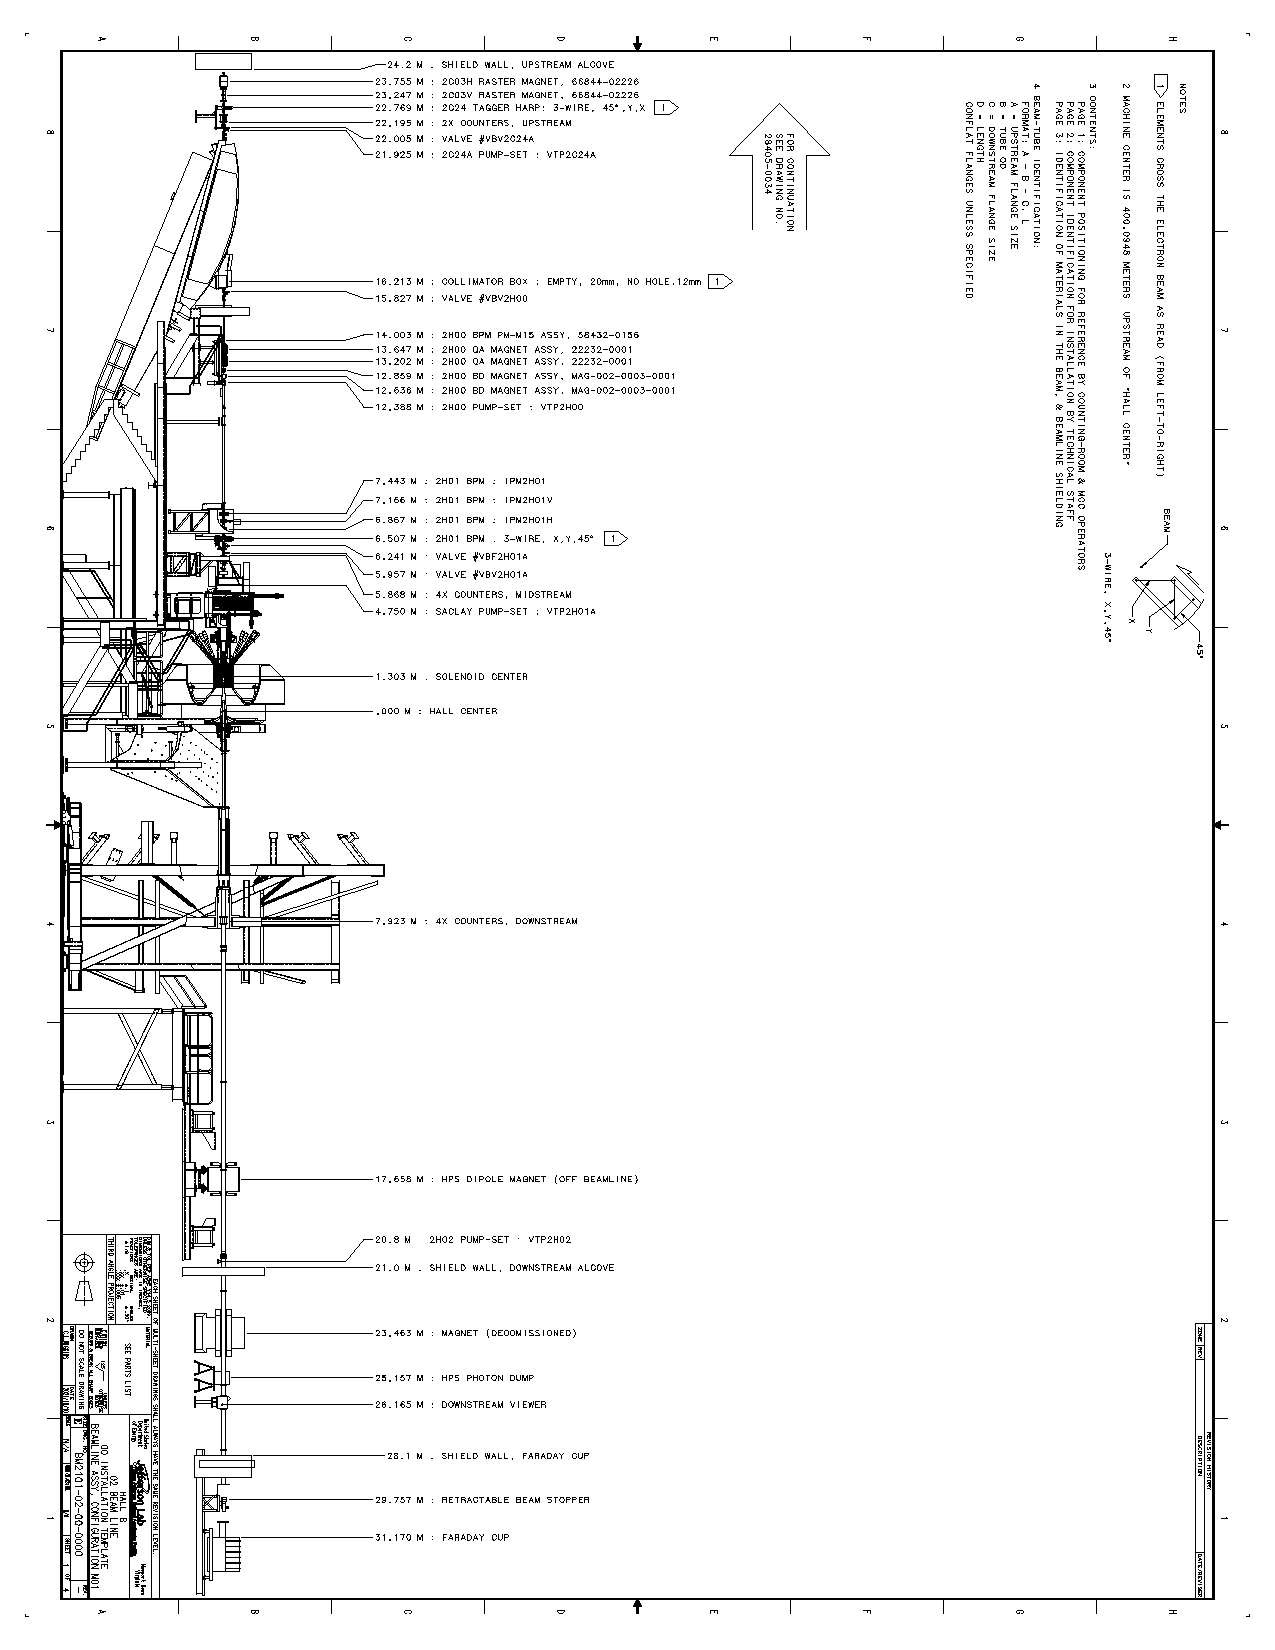
\includegraphics[width=6in]{rgm_beam_page1.pdf}
\caption{ \label{fig:beamline1} The layout of the RG- beamline. }
\end{center}
\end{figure}

\begin{figure}[hbt]
\vspace{-2cm}
\begin{center}
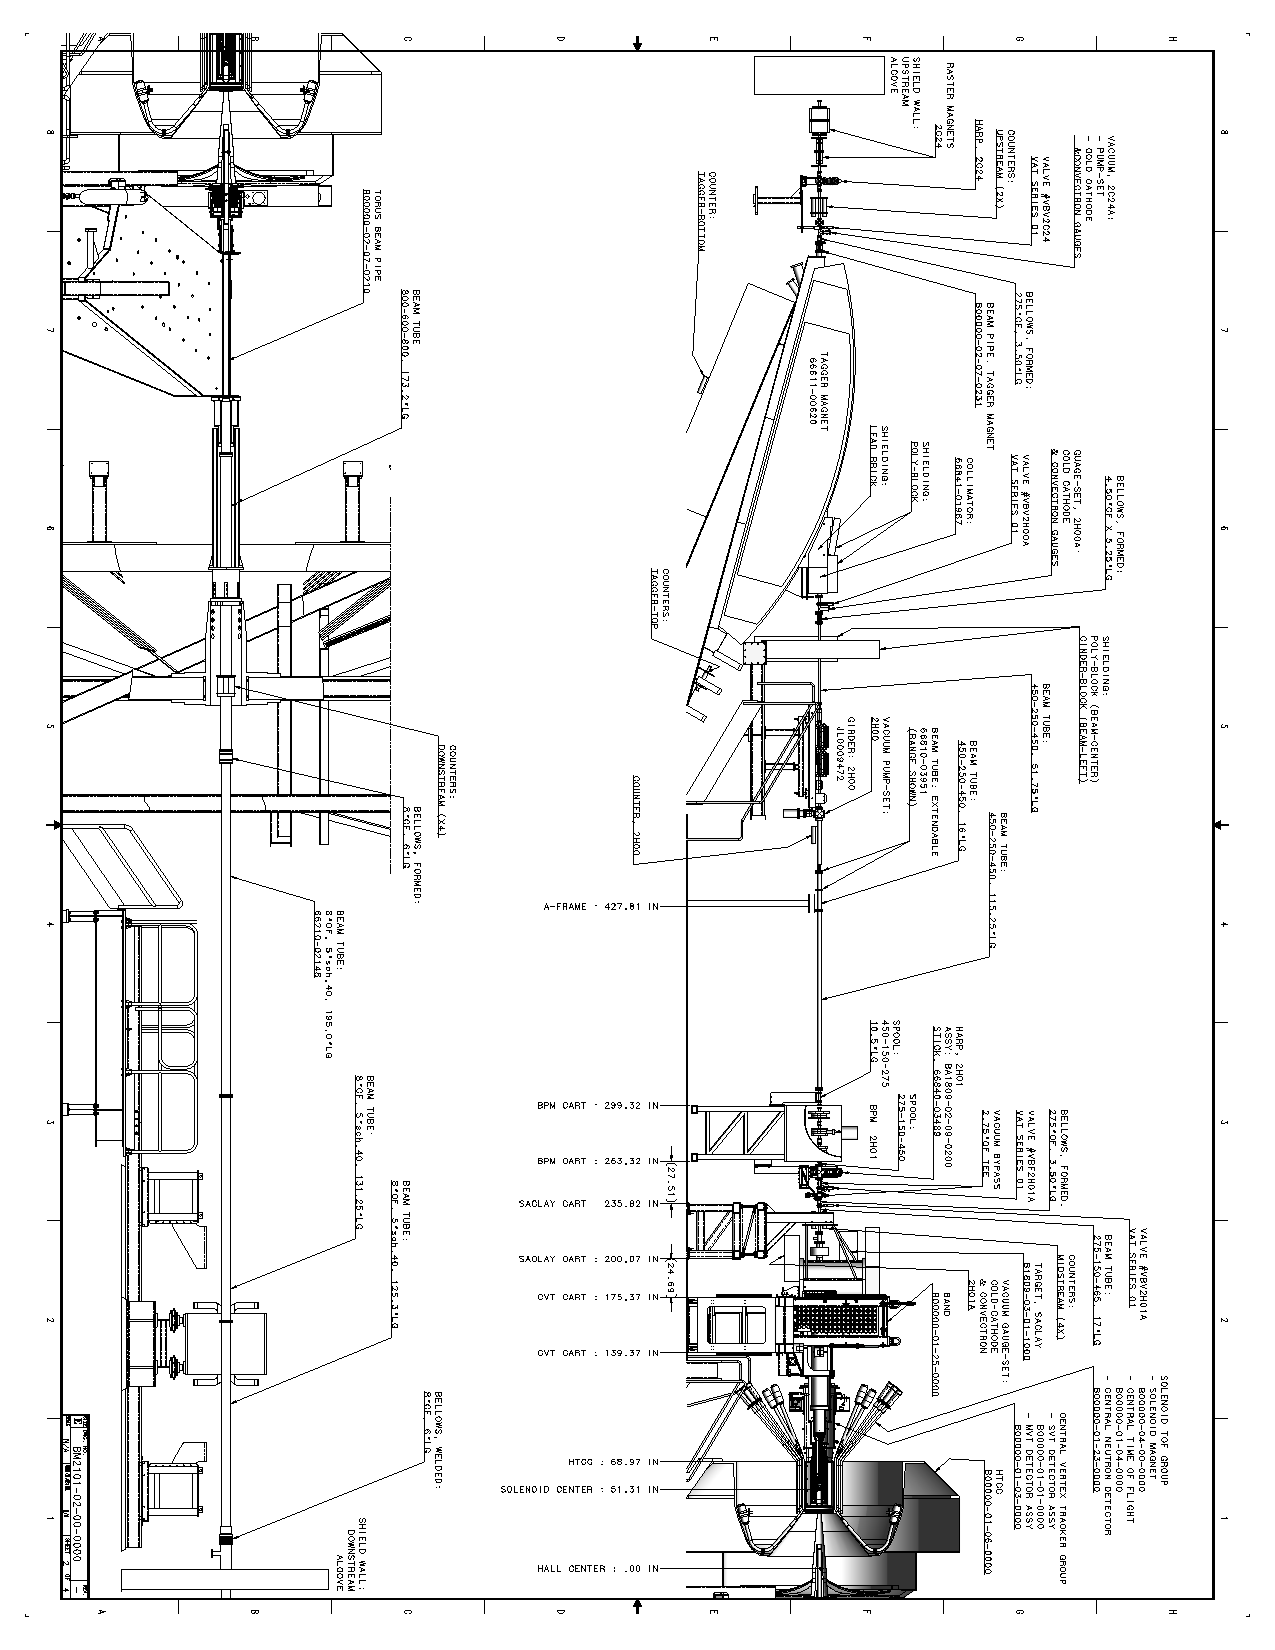
\includegraphics[width=6in]{rgm_beam_page2.pdf}
\end{center}
\caption{ \label{fig:beamline2} 
The layout of the RG-C beamline. }
\end{figure}

\begin{figure}[hbt]
\vspace{-2cm}
\begin{center}
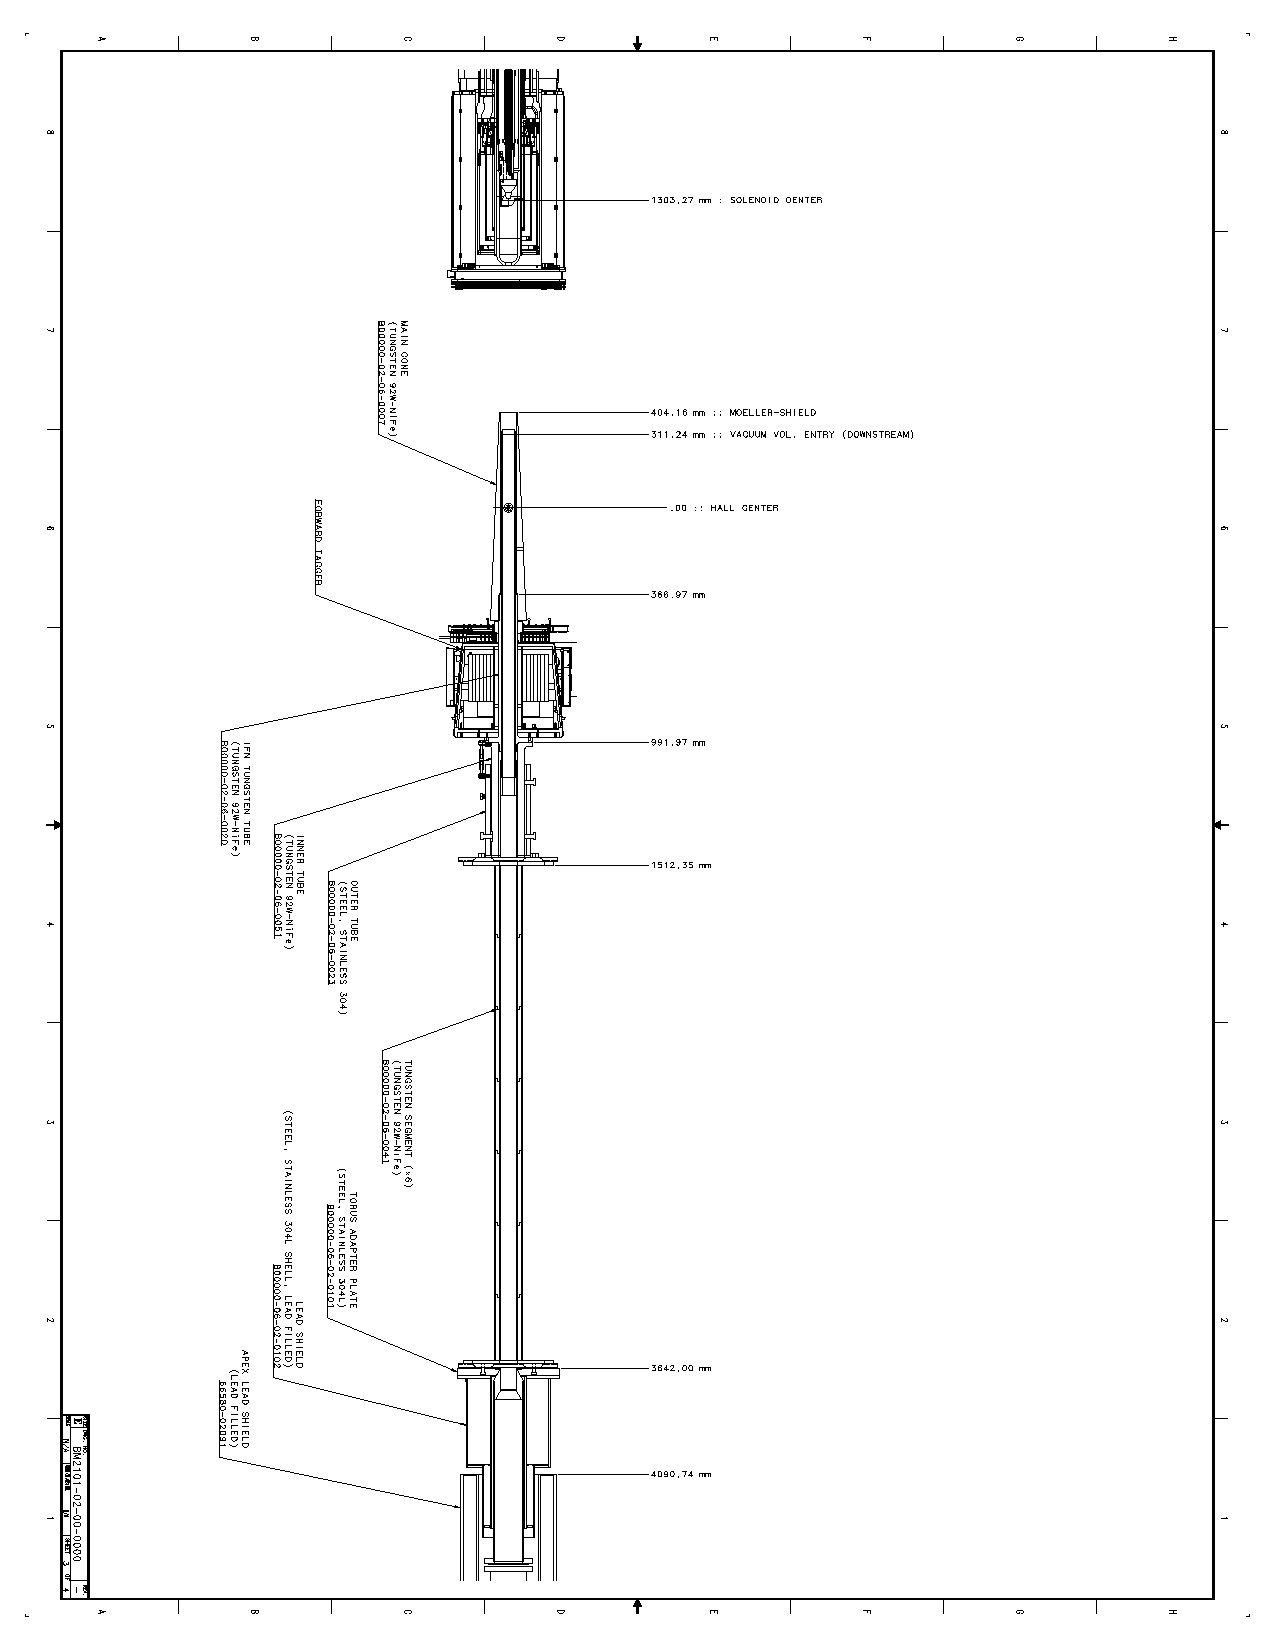
\includegraphics[width=6in]{rgm_beam_page3.pdf}
\end{center}
\caption{ \label{fig:beamline3} 
The layout of the RG-C beamline. }
\end{figure}

\begin{figure}[hbt]
\vspace{-2cm}
\begin{center}
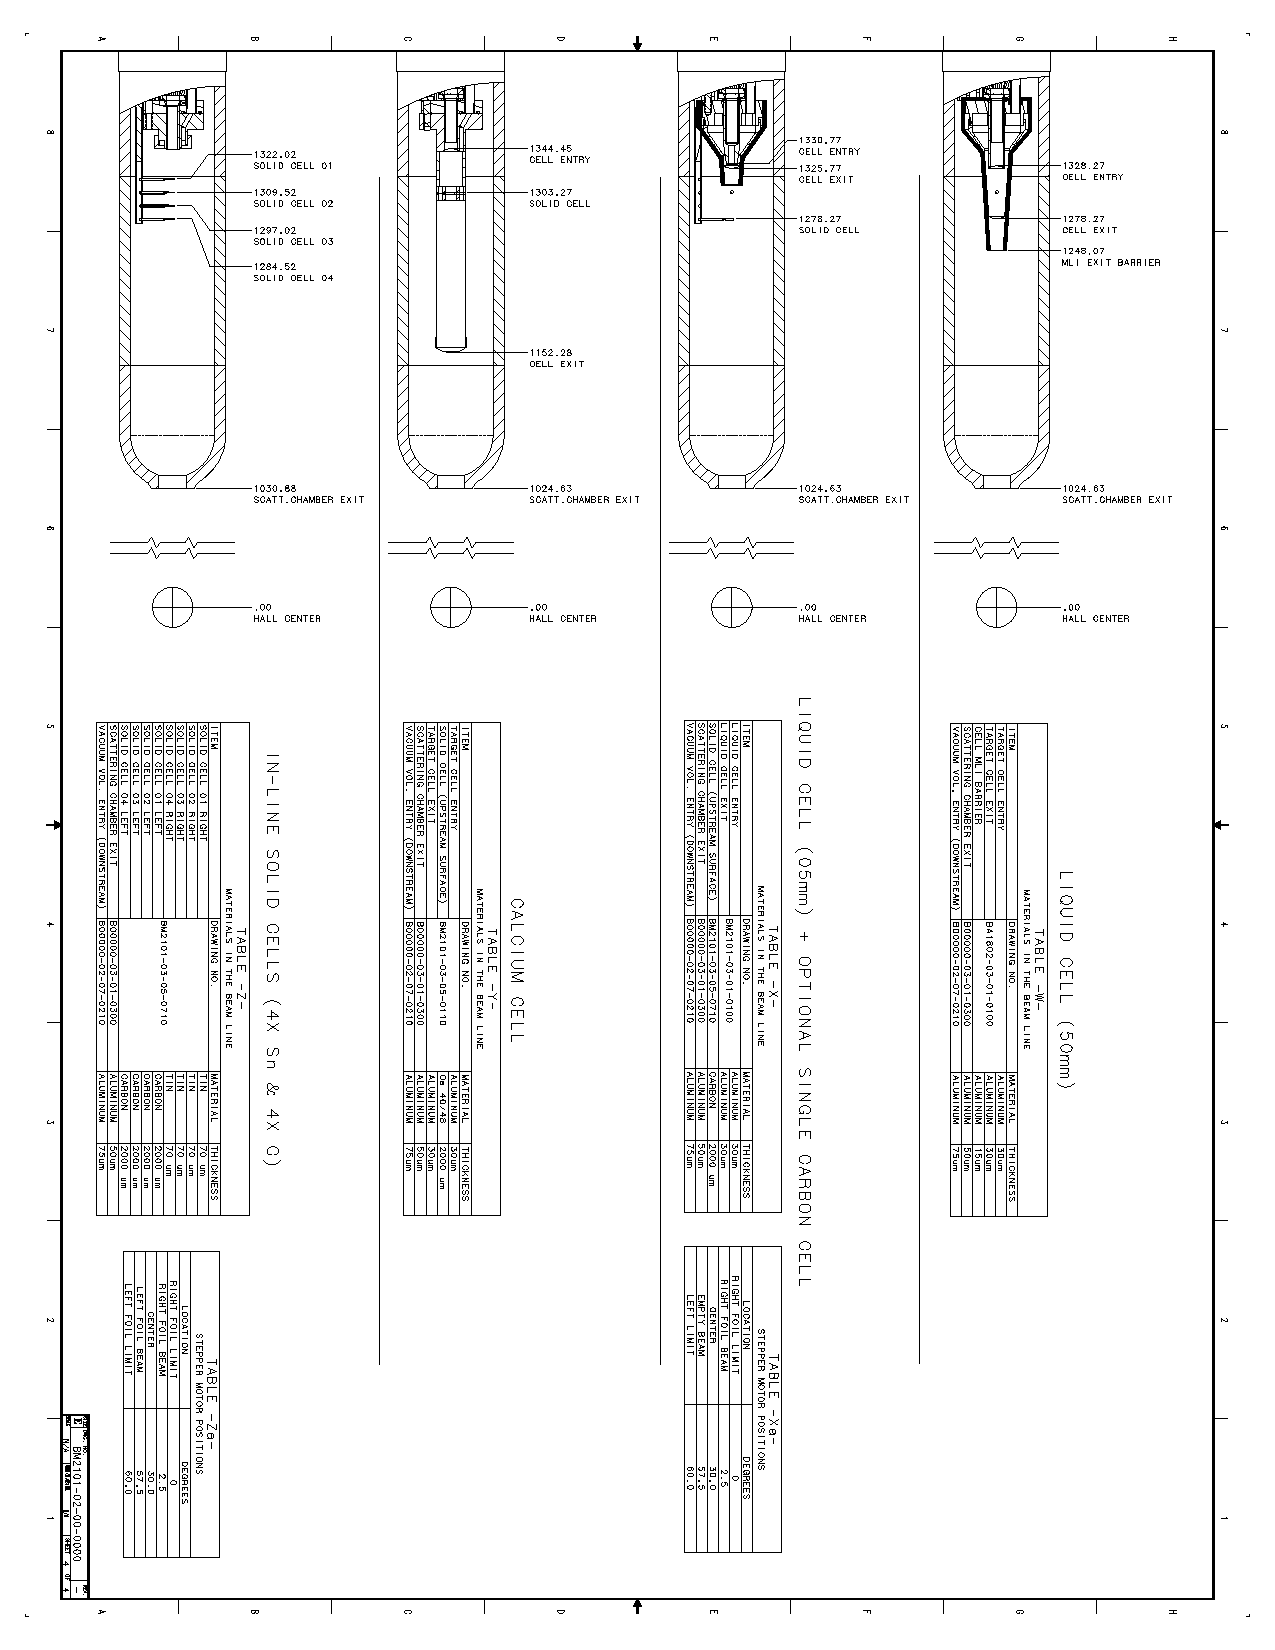
\includegraphics[width=6in]{rgm_beam_page4.pdf}
\end{center}
\caption{ \label{fig:beamline4} 
The layout of the RG-C beamline. }
\end{figure}



%Table~\ref{tab:run_plan} presents the proposed run plan. Depending on the performance of the experiment and accelerator it will be adjusted.

%



\end{document}
